\begin{figure}[t]
\centering
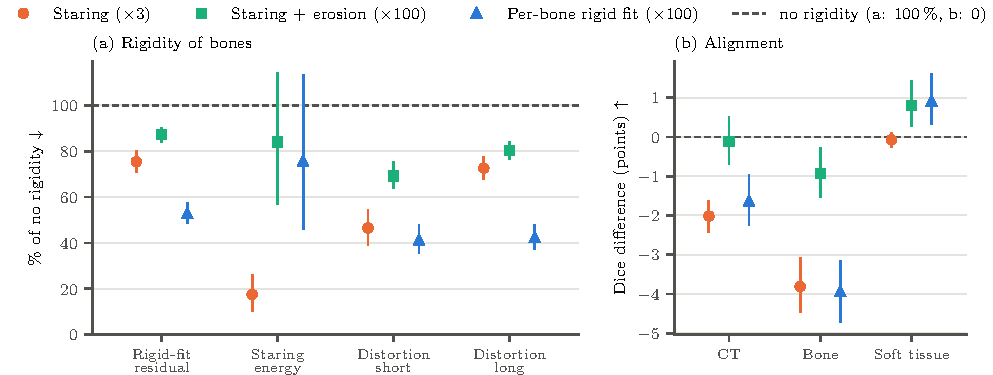
\includegraphics[width=\textwidth]{figures/rigidity_measures.pdf}
\caption{Bone-rigidity penalties evaluated with all bone-rigidity measures on the test set (28 patients, 38 pairs): network trained with the PET-preservation losses, followed by instance optimization (IO) with the PET-preservation terms and one bone-rigidity penalty at the weight chosen on the validation set.
(a)~Bone rigidity relative to IO without bone rigidity (dashed, 100\,\%): residual of a rigid fit to each bone, Staring energy (properness, orthonormality, and affinity) on the whole bone, and distortion of short (5--15~mm) and long ($\geq15$~mm) within-bone distances.
(b)~Change of CT, bone, and soft-tissue Dice relative to IO without bone rigidity.
Color and marker shape identify the bone-rigidity penalty.
Points are means over patients after averaging each patient's pairs; bars are 95\,\% patient-bootstrap confidence intervals.}
\label{fig:rigidity_measures}
\end{figure}
